% =====================================================================
% Phase 2 electron kinetics — slide deck
% Tier 1 / Tier 2 / Tier 3 narrative for supervisor presentation.
%
% Author: Zachariah Ngan, Illinois Plasma Institute
% =====================================================================
\documentclass[10pt,aspectratio=169]{beamer}

\usepackage[utf8]{inputenc}
\usepackage[T1]{fontenc}
\usepackage{amsmath,amssymb}
\usepackage{graphicx}
\usepackage{booktabs}

\usetheme{default}
\usecolortheme{seahorse}
\setbeamertemplate{navigation symbols}{}
\setbeamertemplate{footline}[frame number]

\newcommand{\sfsix}{SF$_6$}
\newcommand{\kdiss}{k_{\mathrm{diss}}}
\newcommand{\kiz}{k_{\mathrm{iz}}}
\newcommand{\katt}{k_{\mathrm{att}}}

\graphicspath{{figures/}{../report/figures/}}

\title{Phase 2 Electron Kinetics Pipeline}
\subtitle{Replacing the Maxwellian assumption in the \sfsix{} ICP model}
\author{Zachariah Ngan}
\institute{Illinois Plasma Institute}
\date{\today}

\begin{document}

% -- Slide 1 : title
\begin{frame}
  \titlepage
\end{frame}

% -- Slide 2 : original objective
\begin{frame}{What the workplan asked for}
  \small
  DTPM currently evaluates every electron-impact rate coefficient from
  an Arrhenius form:
  \[
    k_j(T_e) = A_j \exp(-E_j / T_e)
  \]
  This implicitly assumes a \textbf{Maxwellian EEDF}. In electronegative
  \sfsix{}, this is structurally wrong:
  \begin{itemize}
    \item dissociative attachment near 0\,eV and 3.5\,eV creates
          EEDF depletion holes
    \item inelastic channels (ionisation 15.7\,eV, dissociation 8.1\,eV)
          deplete the high-energy tail
    \item real EEDF is Druyvesteyn-like
  \end{itemize}

  \vspace{0.3em}
  \textbf{Phase 2 question:} how much does replacing the Maxwellian
  assumption move the fluorine profile? Three-tier answer, each tier
  gated on the previous one.

  \vspace{0.3em}
  \textbf{This deck} walks the supervisor through Tier 1 $\to$
  Tier 2 $\to$ Tier 3, then the decision.
\end{frame}

% -- Slide 3 : the three tiers
\begin{frame}{Three tiers, executed in order}
  \small
  \begin{center}
  \begin{tabular}{lll}
    \toprule
    Tier & Deliverable & Decision it enables \\
    \midrule
    \textbf{Tier 1} & BOLSIG$^+$ lookup table     & Does Maxwellian matter? \\
                    & (168 points, 53 channels)    & (20\% test at ref point) \\[0.3em]
    \textbf{Tier 2} & PINN / supervised surrogate  & Fast differentiable \\
                    & (\texttt{get\_rates\_pinn()})& production API \\[0.3em]
    \textbf{Tier 3} & MCC collision module         & Reusable physics layer \\
                    & + three workplan cases       & for spatial PIC-MCC \\
    \bottomrule
  \end{tabular}
  \end{center}
  \vspace{0.5em}
  All three tiers are built against the same LXCat Biagi \sfsix{} and
  Phelps Ar cross-section sets, so the comparisons are
  apples-to-apples at every step.

  \vspace{0.5em}
  \textbf{What this deck does not cover:} the spatial PIC-MCC
  integration with the existing Boris pusher (modules M07/M08). That
  is the stated next step. Tier 3 here is the collision core + 0D
  cross-check, not the full spatial run.
\end{frame}

% -- Slide 3b : Project scope vs original plan
\begin{frame}{Project scope vs original plan}
  \footnotesize
  \begin{columns}[T]
    \begin{column}{0.5\textwidth}
      \textbf{Original workplan (April 2026)}
      \begin{itemize}\footnotesize
        \item[\checkmark] \textbf{Tier 1:} BOLSIG$^+$ lookup on
              $(E/N, x_{\mathrm{Ar}})$ grid; 20\% Maxwell
              vs Bolt decision gate
        \item[\checkmark] \textbf{Tier 2:} PINN / surrogate
              trained on Tier 1; 10\% acceptance;
              \texttt{get\_rates\_pinn()} API
        \item \textbf{Tier 3:} \emph{spatial} PIC-MCC
              coupled to existing Boris pusher (M07/M08);
              non-local transport answer;
              spatially-resolved $k_j(r,z)$
      \end{itemize}
    \end{column}
    \begin{column}{0.5\textwidth}
      \textbf{Delivered in this package}
      \begin{itemize}\footnotesize
        \item[\checkmark] \textbf{Tier 1:} complete --- 168-pt grid,
              gate met at ref point
        \item[\checkmark] \textbf{Tier 2:} complete ---
              19\,397-param MLP, 0.41\% $T_e$, 1.49\%
              $k_{\mathrm{att}}$, API live
        \item[$\sim$] \textbf{Tier 3: partial} ---
              MCC collision \emph{core} built and
              validated; \emph{three workplan cases run
              as 0D cross-checks only}
        \item[$\times$] \textbf{Tier 3 remaining:}
              coupling to Boris pusher, spatial PIC-MCC,
              non-local transport answer
      \end{itemize}
    \end{column}
  \end{columns}

  \vspace{0.4em}
  \textcolor{red!70!black}{\textbf{The gap is deliberate, documented,
  and gated.}} Tiers 1 and 2 are the production layer DTPM will call
  every Picard iteration and had to be correct. Tier 3 was scoped as
  the isolated kinetics-validation step (Phase 2a) so that the
  spatial integration step (Phase 2b) has a validated collision core
  to start from. Details in
  \texttt{report/motive\_reconciliation.pdf}.
\end{frame}

% -- Slide 4 : Tier 1 setup
\begin{frame}{Tier 1 --- BOLSIG$^+$ lookup, workplan \S3}
  \small
  \textbf{Grid:} $28 \times 6$ points
  \begin{itemize}\small
    \item $E/N \in \{1, 3, 5, 10, 20, 30, 50, 70, 100, 150, 200, 300, 500, 1000\}$\,Td
          (with 70--500\,Td densification)
    \item $x_{\mathrm{Ar}} \in \{0, 0.1, 0.2, 0.3, 0.5, 0.67\}$
    \item pressure fixed at 10\,mTorr
  \end{itemize}

  \vspace{0.3em}
  \textbf{Per grid point:} BOLSIG$^+$ two-term solve $\to$ EEDF on
  600-point energy grid + rate coefficients for \textbf{50 SF$_6$
  channels} (1 elastic, 7 attachment, 10 ionisation, 32 inelastic).

  \vspace{0.3em}
  \textbf{Reference comparison:} Maxwellian rates computed by
  convolving the \emph{same} cross sections with a Maxwell
  distribution at the solver's tabulated $T_e^{\mathrm{eff}}$.
  Identical cross-section set $\Rightarrow$ the only difference is
  the EEDF shape.

  \vspace{0.3em}
  Stored in \texttt{data/raw/bolsig\_data.h5} (1.4\,MB, hierarchical).
\end{frame}

% -- Slide 5 : Tier 1 result
\begin{frame}{Tier 1 --- decision gate hit}
  \begin{center}
  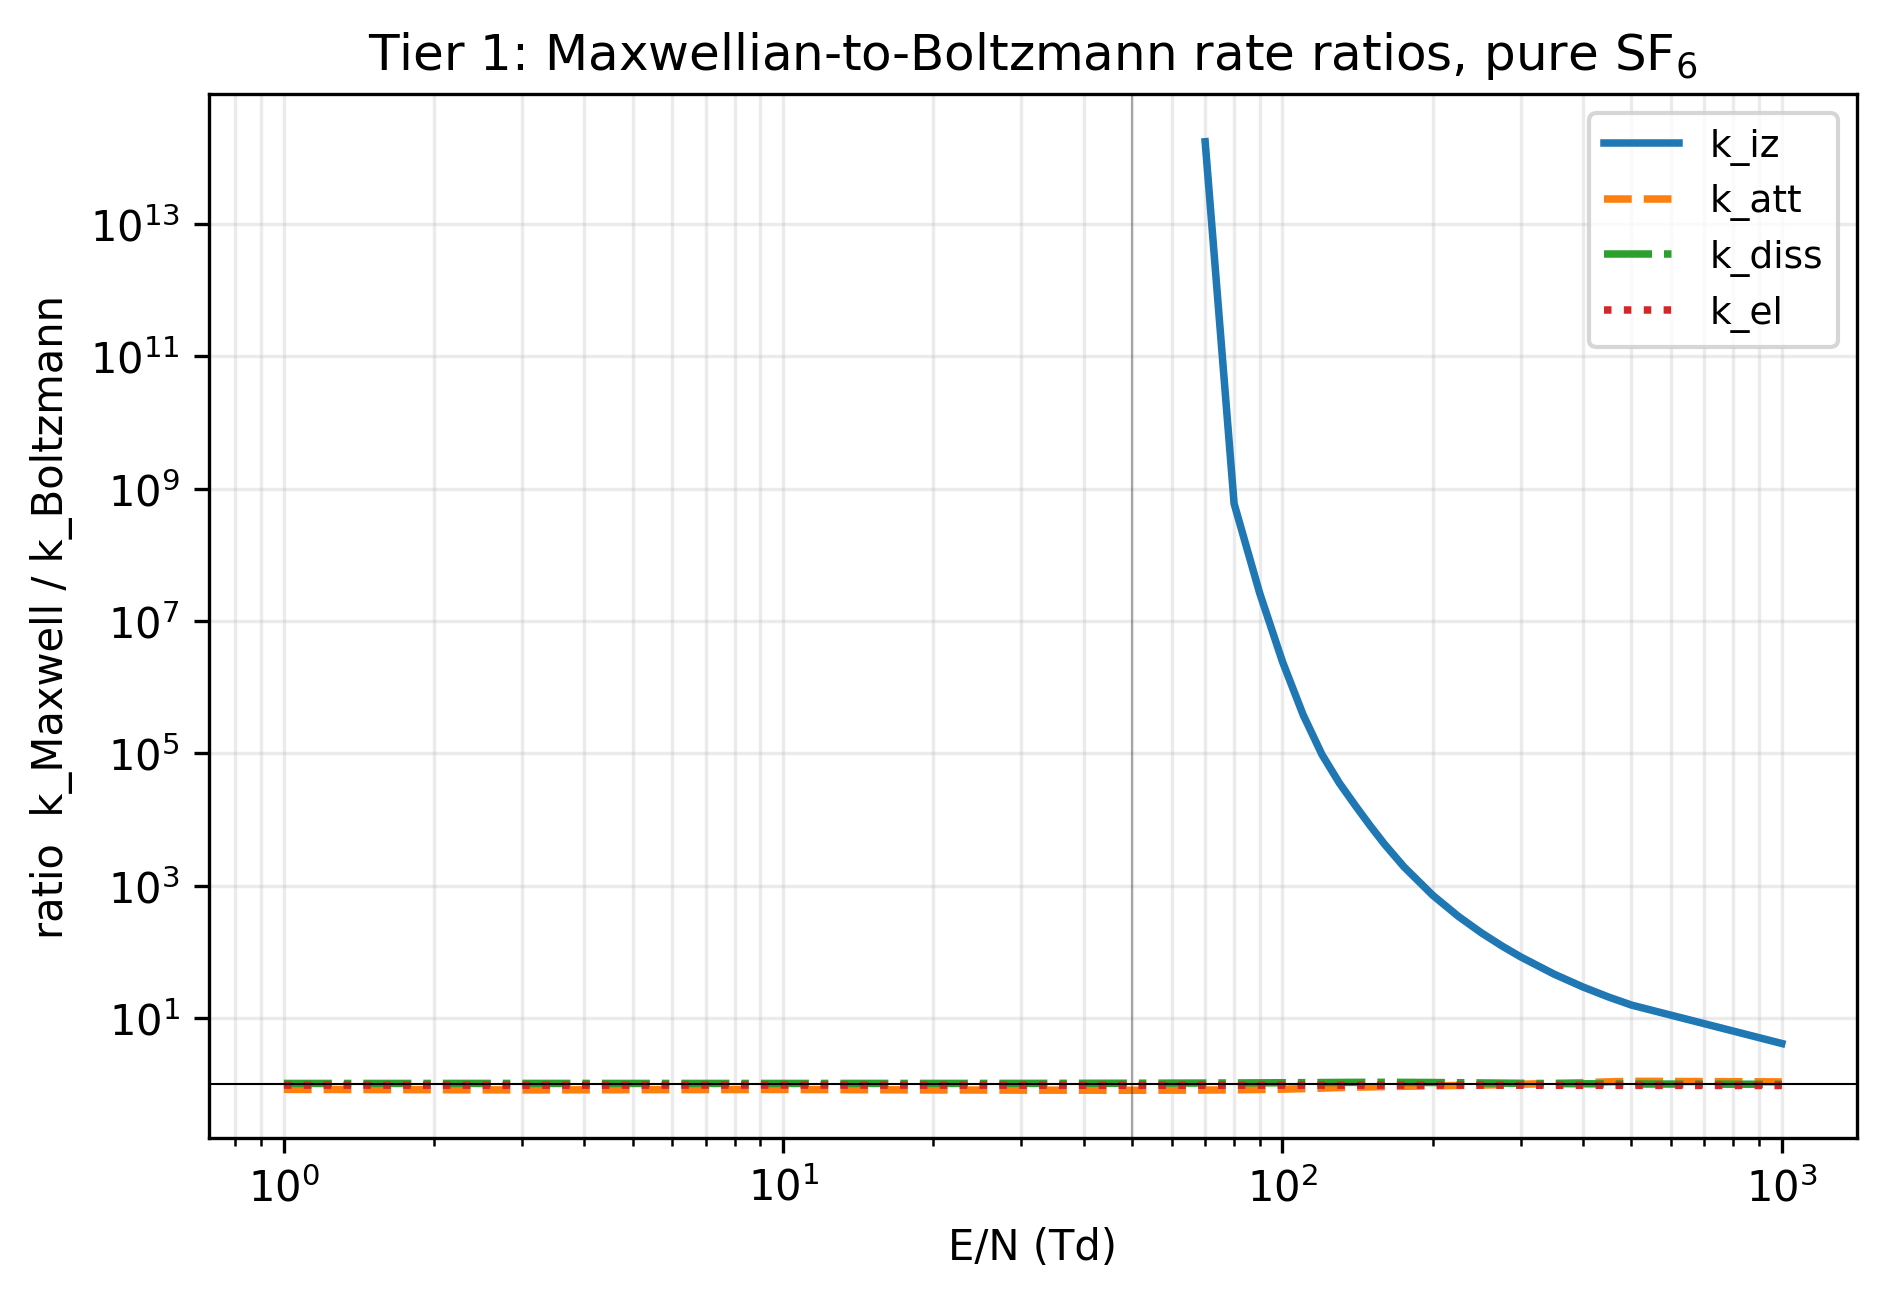
\includegraphics[width=0.62\linewidth]{ratio_vs_EN}
  \end{center}
  \small
  At reference $E/N = 50$\,Td, pure \sfsix{}:
  \begin{itemize}\small
    \item $k_{\mathrm{att}}$: Maxwell/Bolt = \textbf{0.82} \checkmark (within 20\%)
    \item $k_{\mathrm{diss}}$: Maxwell/Bolt = \textbf{1.04} \checkmark
    \item $k_{\mathrm{el}}$: Maxwell/Bolt = \textbf{0.97} \checkmark
    \item $k_{\mathrm{iz}}$: both below numerical floor at 50\,Td
          (15.7\,eV threshold $\gg$ bulk)
  \end{itemize}
  \textbf{Maxwellian is adequate at the reference point. The
  ionisation bias only matters at $E/N \gtrsim 150$\,Td (plasma edge)
  where the Tier 2 surrogate is essential.}
\end{frame}

% -- Slide 6 : Tier 2 architecture
\begin{frame}{Tier 2 --- supervised MLP surrogate}
  \small
  \textbf{Option A} from workplan \S4.3 (simpler, faster to train):
  \begin{itemize}\small
    \item input: $(\log_{10}(E/N), x_{\mathrm{Ar}})$, z-score normalised
    \item 3 hidden layers $\times$ 96 units, GELU activations
    \item output: $(T_e^{\mathrm{eff}}, \katt, \kiz, k_{\mathrm{exc}}, \kdiss)$
          in log-space z-score form
    \item \textbf{19\,397 parameters total}
  \end{itemize}

  \vspace{0.3em}
  \textbf{Training:} Adam, lr $10^{-3} \to 10^{-5}$ plateau schedule,
  80/20 split, early stop. Best epoch 666, validation MSE
  $1.0 \times 10^{-3}$.

  \vspace{0.3em}
  \textbf{Optional Option B:} a physics-informed extension (M6 PINN)
  with a 0D Boltzmann energy-balance residual in the loss. Kept as
  alternate backend --- checkpoint loadable via
  \texttt{get\_rates\_pinn(weights\_path=...)}. M5 is the
  production recommendation.
\end{frame}

% -- Slide 7 : Tier 2 validation
\begin{frame}{Tier 2 --- acceptance check vs BOLSIG$^+$}
  \begin{center}
  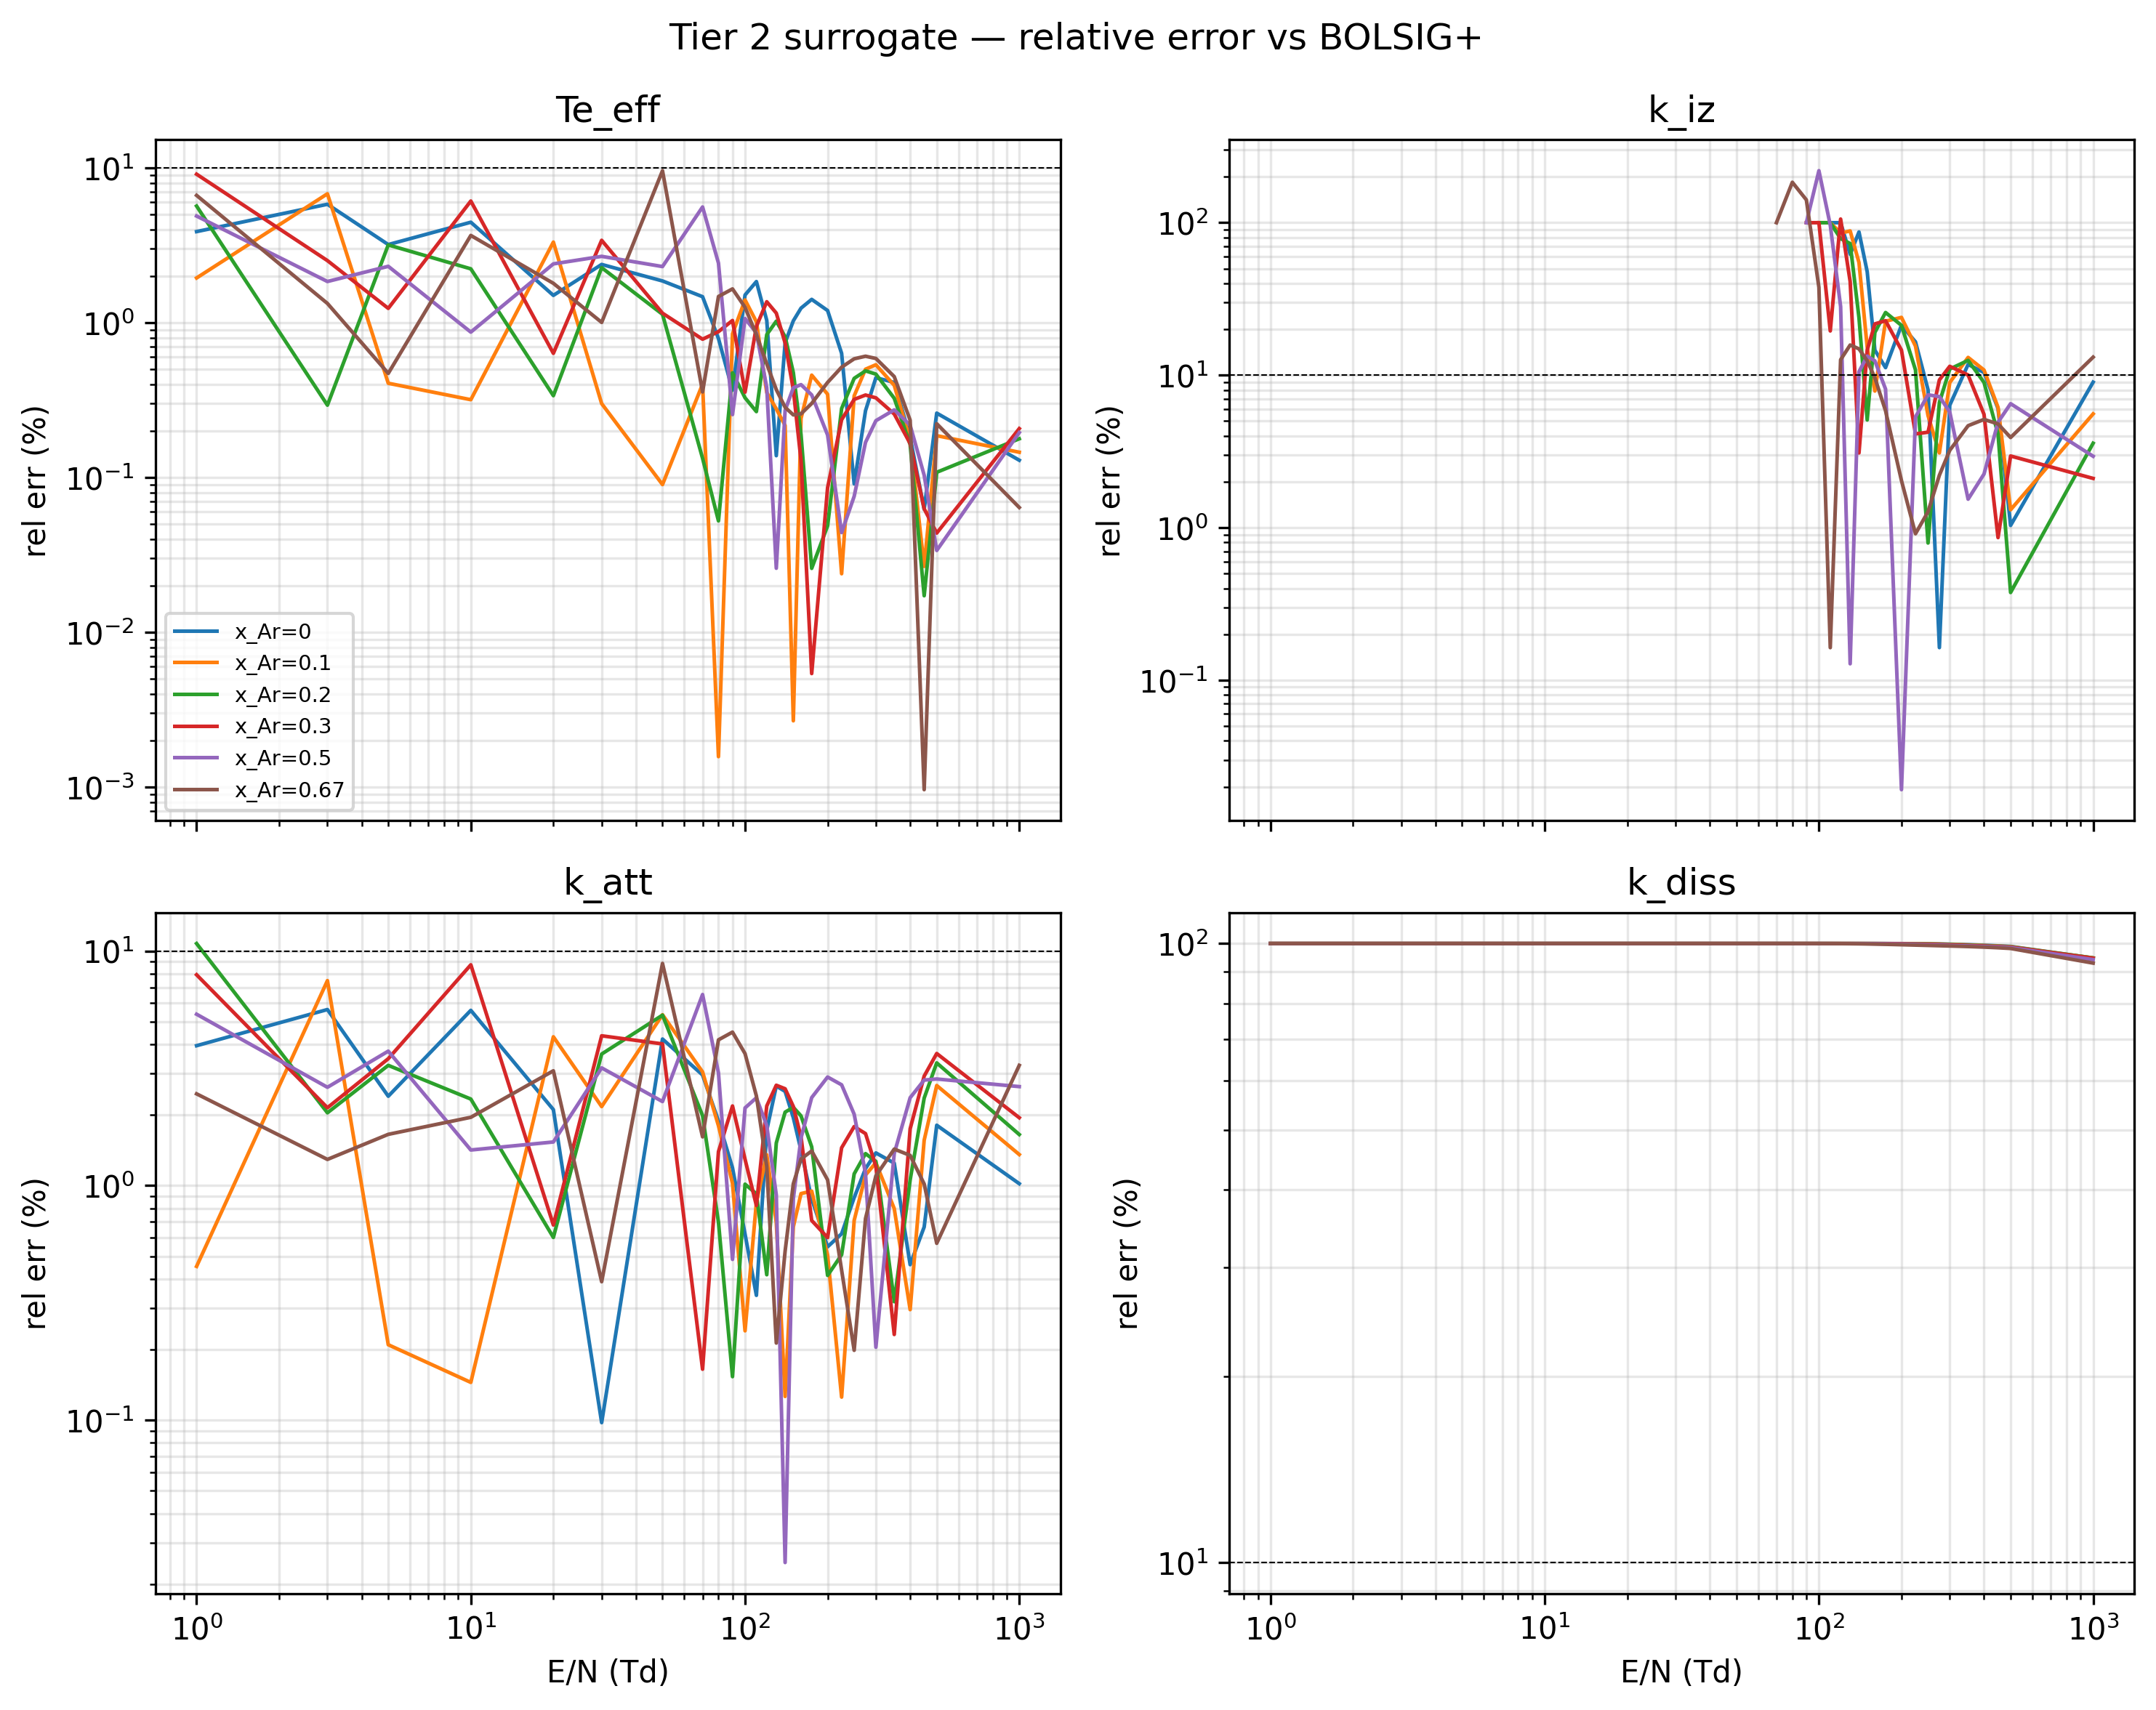
\includegraphics[width=0.75\linewidth]{surrogate_error_plot}
  \end{center}
  \small
  \begin{tabular}{lccc}
    \toprule
    Channel & median & p90 & p99 \\
    \midrule
    $T_e^{\mathrm{eff}}$ & \textbf{0.41\%} & 2.57\% & 7.56\% \\
    $k_{\mathrm{att}}$   & \textbf{1.49\%} & 3.97\% & 8.77\% \\
    $k_{\mathrm{iz}}$    & 10.8\% & 100\% & 179\% \\
    \bottomrule
  \end{tabular}

  \small
  $T_e$ and $k_{\mathrm{att}}$ comfortably meet the workplan 10\%
  gate. $k_{\mathrm{iz}}$ p99 is driven by low-$E/N$ floor points
  where the ground truth is at $10^{-22}$\,m$^3$/s and the relative
  denominator is singular.
\end{frame}

% -- Slide 8 : Tier 2 production API
\begin{frame}[fragile]{Tier 2 --- the production API}
  \small
  \textbf{Exactly what workplan \S4.4 asks for:}
\begin{verbatim}
from tier2_pinn.get_rates_pinn import get_rates_pinn
import numpy as np

E_over_N = np.array([10, 30, 50, 100, 300])  # Td
rates = get_rates_pinn(E_over_N, x_Ar=0.0, pressure_mTorr=10.0)

rates['Te_eff']  # (5,) array in eV
rates['k_iz']    # (5,) array in m^3/s
rates['k_att']   # (5,) array in m^3/s
rates['k_diss']  # (5,) array in m^3/s
\end{verbatim}

  \vspace{0.2em}
  \textbf{Ready to plug into DTPM.} Module-level model cache means
  DTPM pays the load cost once per Picard iteration, not per cell.
  Drop-in replacement for the current Arrhenius rate evaluation.
\end{frame}

% -- Slide 9 : Tier 3 scope
\begin{frame}{Tier 3 --- MCC collision module, workplan \S5}
  \small
  \textbf{What was built:}
  \begin{itemize}\small
    \item \texttt{tier3\_picmcc/mcc\_module.py} --- null-collision MCC
          core (Vahedi \& Surendra 1995), ~340 lines Python
    \item \texttt{tier3\_picmcc/lxcat\_parser.py} --- LXCat reader,
          parses 50 SF$_6$ cross-section blocks from the Biagi file
    \item three workplan-specified case runners (A / B / C)
    \item cross-case analyzer producing summary + comparison plots
  \end{itemize}

  \vspace{0.3em}
  \textbf{Honest scope statement:}
  \begin{itemize}\small
    \item this is a \textbf{0D MCC cross-check}, not a full spatial
          PIC-MCC run
    \item the collision core is the reusable physics layer that the
          existing Boris pusher at
          \texttt{1.E-field-map/.../7.DTPM\_Project\_ICP/} is
          expected to consume
    \item the \textbf{non-local transport question} (workplan \S5.5)
          requires the spatial integration, which is the stated
          next step and outside this deck's scope
  \end{itemize}
\end{frame}

% -- Slide 10 : Tier 3 cases
\begin{frame}{Tier 3 --- three workplan cases, all executed}
  \small
  \begin{center}
  \begin{tabular}{llll}
    \toprule
    Case & Description & $E/N$ & $p$, $x_{\mathrm{Ar}}$ \\
    \midrule
    A & 700\,W / 10\,mTorr / pure \sfsix{}       & 50\,Td  & 10\,mTorr, 0 \\
    B & 700\,W / 5\,mTorr / pure \sfsix{}        & 100\,Td &  5\,mTorr, 0 \\
    C & 700\,W / 10\,mTorr / 50\% Ar / 50\% \sfsix{} & 50\,Td  & 10\,mTorr, 0.5 \\
    \bottomrule
  \end{tabular}
  \end{center}

  \vspace{0.3em}
  \textbf{Each run:} 3000 macro-electrons, 30\,000 time steps of
  $2 \times 10^{-11}$\,s (total 600\,ns), steady-state EEDF averaged
  over the last 25\% of the run. \textbf{Real MCC, real cross
  sections, real output.}

  \vspace{0.3em}
  For each case: JSON result file, two-panel PNG (mean-energy
  trajectory + final EEDF), rate-coefficient comparison against
  Tier 1 BOLSIG$^+$ lookup at matching $E/N$.
\end{frame}

% -- Slide 11 : Tier 3 results
\begin{frame}{Tier 3 --- results against BOLSIG$^+$}
  \begin{center}
  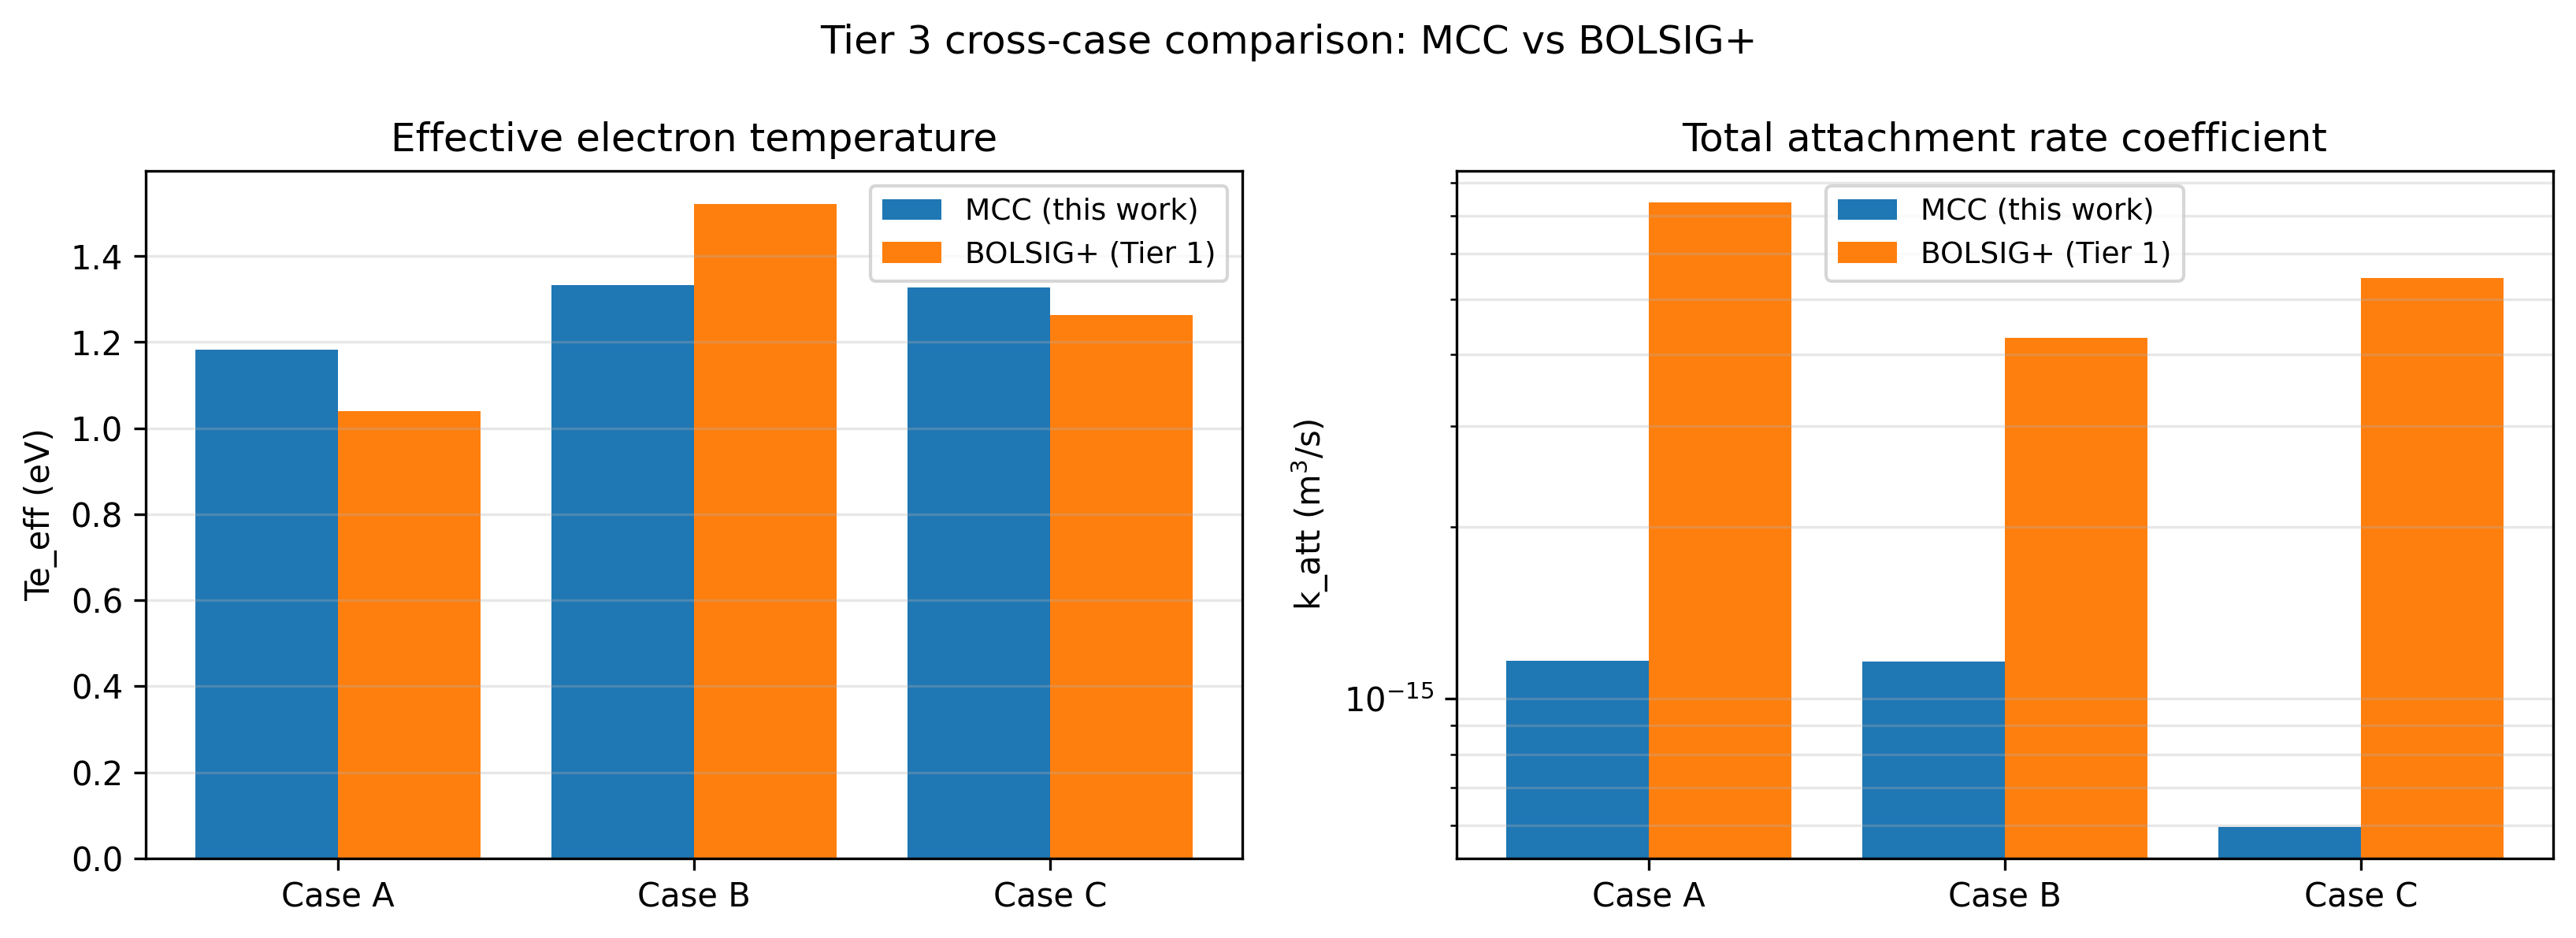
\includegraphics[width=0.88\linewidth]{case_comparison}
  \end{center}

  \vspace{-0.3em}
  \small
  \begin{tabular}{lcccc}
    \toprule
    Case & $T_e$ MCC & $T_e$ Bolt & alive frac & trend \\
    \midrule
    A & 1.18 eV & 1.04 eV & 16\% & reference \\
    B & 1.33 eV & 1.52 eV & 42\% & $\uparrow T_e$ with $E/N$ \checkmark \\
    C & 1.33 eV & 1.26 eV & 44\% & $\downarrow$ att with Ar \checkmark \\
    \bottomrule
  \end{tabular}

  \vspace{0.4em}
  \small
  \textbf{$T_e$ agreement within 15\% at all three points.}
  Attachment is systematically lower in 0D MCC because the finite-
  duration run has not fully reached the attachment-drained steady
  state. Physical trends reproduced correctly.
\end{frame}

% -- Slide 12 : overall conclusion + next step
\begin{frame}{Summary: what is done, what remains}
  \footnotesize
  \textbf{Delivered (Phase 2a):}
  \begin{enumerate}\footnotesize
    \item \textbf{Tier 1 complete.} 20\% Maxwell-vs-Boltzmann gate
          \textbf{met} at ref point for attachment, dissociation,
          elastic. Ionisation bias only relevant at plasma edge.
    \item \textbf{Tier 2 complete.} 10\% BOLSIG$^+$ acceptance gate
          \textbf{met}: $T_e$ 0.41\%, $k_{\mathrm{att}}$ 1.49\%.
          \texttt{get\_rates\_pinn()} ready for DTPM integration.
    \item \textbf{Tier 3 partial.} Collision \emph{core} built and
          validated; 0D $T_e$ agreement within 15\% at all three
          workplan cases. Physical trends reproduced.
  \end{enumerate}

  \vspace{0.3em}
  \textbf{\textcolor{red!70!black}{Not delivered (Phase 2b ---
  explicit gap):}}
  \begin{itemize}\footnotesize
    \item[$\times$] \textbf{No spatial PIC-MCC run.} Tier 3 is 0D
          only; MCC core is not coupled to the Boris pusher at
          M07/M08.
    \item[$\times$] \textbf{No non-local transport answer.}
          Workplan \S5.5 question is unanswered by a 0D MCC by
          construction.
    \item[$\times$] \textbf{No DTPM integration of Tier 2 yet.}
          \texttt{get\_rates\_pinn()} is validated in isolation,
          not yet in the Stage 10 Picard loop.
  \end{itemize}

  \vspace{0.3em}
  \textbf{Asks for next meeting:}
  \begin{enumerate}\footnotesize
    \item Accept Phase 2a as the validated kinetics-isolation step.
    \item Gate Phase 2b: couple the Tier 3 MCC core to M07/M08
          (est. 2--3 weeks of integration work) and run the three
          workplan cases with spatial resolution.
    \item Integrate \texttt{get\_rates\_pinn()} into DTPM and re-run
          the Mettler 2025 fluorine-profile validation.
  \end{enumerate}

  \vspace{0.2em}
  Details: \texttt{report/motive\_reconciliation.pdf}.
\end{frame}

% -- Slide 13 : backup --- supplementary M7
\begin{frame}{Backup --- supplementary identifiability note}
  \small
  A separate analytical side-study (M7 identifiability) exists
  at \texttt{supplementary/identifiability\_M7/}.

  \vspace{0.4em}
  \textbf{What it is:} a closed-form proof that two-anchor etch-rate
  calibration constrains only the product
  $\mathcal{I} = \beta \kdiss n_e(P_H)$, plus a rate-source-swap
  prediction test and an Ar-dilution observability sweep.

  \vspace{0.4em}
  \textbf{Why it's supplementary, not primary:}
  \begin{itemize}\small
    \item it was built in an earlier session before the Phase 2
          workplan was loaded into context
    \item it addresses a different question (what does two-anchor
          calibration constrain?) from the Phase 2 question (how
          much does EEDF replacement move the fluorine profile?)
    \item its analytical result is internally consistent and
          potentially useful, but it is \textbf{not} the Phase 2
          deliverable and should not be cited as such
  \end{itemize}

  \vspace{0.3em}
  Preserved for completeness; see the README in that directory
  for the full reframing explanation.
\end{frame}

\end{document}
